\section{Delay, several channels and several bands}\label{sec:beyond}

This section takes up the questions left by
\cref{sec:pointwise,sec:allzeros}: a lead combined with a delay, a delay
combined with zeros, matrix phases and several bands. For an affine phase without zeros the least mean loss is found
exactly for every slope. A delay can beat the delayed optimum
$e^{i\tau z}\Hs_\theta$, and for a delay there is no system that is optimal at
every frequency at once. For matrix phases there is in general no least
attenuation in the Loewner order, but the least trace is explicit. With
zeros allowed and a delay, the optimum exists and is unique, and its loss
falls off exponentially in the delay, while without zeros it stays above a
fixed positive floor.\footnote{\Cref{thm:exactmean,thm:delay,thm:trace,thm:noloewner,thm:multiband}
and \cref{lem:meandual,lem:multicomp} were found with OpenAI's ChatGPT,
starting from \cref{thm:reconstruction,thm:allzeros}; every number was
recomputed (\cref{app:verification}).}

\subsection{A lead with a delay}\label{ssec:exactmean}

Fix $s>0$ and $\tau\in\R$, and let $\mathcal M_s(\tau)$ be the infimum of
$\frac1{b-a}\int_a^b\alpha$ over the zero-free passive systems, regular on the
band, with phase $-s+\tau\omega$. For $\tau\le0$ it is given by
\cref{thm:leadpoint}. For $y\ge0$ put
\begin{equation}\label{eq:qdef}
q(y)=\frac2\pi\int_a^b\frac{\sqrt y}{\sqrt y+t}\,\frac{\dd t}{r(t)} .
\end{equation}

\begin{lemma}\label{lem:q}
$q(0)=0$, $q(y)\to\tau_\circ$ as $y\to\infty$, $q'>0$ and $q''<0$ for $y>0$,
and $q(x^2)=xA(x)/r(x)$ for $a<x<b$.
\end{lemma}

\begin{proof}
The function $y\mapsto\sqrt y/(\sqrt y+t)$ is increasing and strictly concave
for $t>0$, and $\frac2\pi\int_a^b\dd t/r=\tau_\circ$. By
\cref{prop:profile}(ii) for $g=1$ and \eqref{eq:affinehg},
$xA(x)/r(x)=\frac{2x^2}\pi\PV\int_a^b\dd t/((x^2-t^2)r(t))$. Glauert's
integral in $\sigma=t^2$ (proof of \cref{lem:positivity}) says
$\PV\int_a^b2t\dd t/((x^2-t^2)r)=0$, that is,
$\PV\int\dd t/((x-t)r)=\int\dd t/((x+t)r)$; with
$2x^2/(x^2-t^2)=x/(x-t)+x/(x+t)$ this gives $q(x^2)$.
\end{proof}

So $A=(r/x)\,q(x^2)$ on the band. Put
\begin{gather*}
f=\frac{a+b}2,\quad \ell=\frac{b-a}2,\quad
\Gamma_0=\pi\ell^2=\int_a^b\frac{r(x)}x\dd x,\\
\tau_c=s\,\big(\tau_\circ-q(b^2)\big)=\frac{2s}\pi\int_a^b\frac{t\dd t}{(b+t)\,r(t)}>0 .
\end{gather*}
For $u<a^2$ and $v>b^2$ let
\begin{align*}
\Gamma_-(u)&=\int_a^b\frac{x\,r(x)}{x^2-u}\dd x\\
&=\frac\pi2\Big(\frac{a^2+b^2}2-u-\sqrt{(a^2-u)(b^2-u)}\Big),\\
\Gamma_+(v)&=\int_a^b\frac{x\,r(x)}{v-x^2}\dd x\\
&=\frac\pi2\Big(v-\frac{a^2+b^2}2-\Delta(v)\Big),
\end{align*}
$\Delta(v)=\sqrt{(v-a^2)(v-b^2)}$; both follow from $\sigma=x^2$ and
$\sigma=\frac{a^2+b^2}2-\frac{b^2-a^2}2\cos\phi$, as in the proof of
\cref{cor:pointwisecons}(iv), and $\Gamma_-(0)=\Gamma_0$. Finally, for
$v>b^2$,
\begin{gather*}
x(v)=\frac{v-\Delta(v)+ab}{a+b},\\
\Phi(v)=\tau_\circ-q\big(x(v)^2\big)+q'\big(x(v)^2\big)\big(v-x(v)^2\big).
\end{gather*}

\begin{theorem}\label{thm:exactmean}
Let $s>0$.
\begin{enumerate}
\item[(i)] If $\tau\le\tau_c$, every zero-free passive system regular on the
band with phase $-s+\tau\omega$ satisfies
\[
\alpha(x)\ge\frac{r(x)}x\big(s\tau_\circ-\tau-s\,q(x^2)\big)\ge0
\qquad(a\le x\le b),
\]
with equality throughout the band for $h=-sh_\circ+\tau z+(s\tau_\circ-\tau)R/z$,
and equality at one point of $(a,b)$ forces this $h$. Hence
$\mathcal M_s(\tau)=-s\Lambda+\frac\pi4(b-a)(s\tau_\circ-\tau)$.
\item[(ii)] If $\tau>\tau_c$, there is exactly one $v>b^2$ with
$s\Phi(v)=\tau$. With $x_*=x(v)$, $y_*=x_*^2$,
\begin{align*}
D&=s\,q'(y_*)\,\frac{(v-y_*)^2}v,\\
C&=s\Big(q(y_*)-q'(y_*)\,\frac{y_*(v-y_*)}v\Big),
\end{align*}
one has $C>0$, $D>0$, $f<x_*<b$, the function
\begin{equation}\label{eq:hexact}
h_{\rm opt}=-sh_\circ+\tau z+R(z)\Big(\frac Cz+\frac{Dz}{v-z^2}\Big)
\end{equation}
is the Herglotz function of an admissible system, and
\begin{equation}\label{eq:exactmean}
\mathcal M_s(\tau)=-s\Lambda+\frac{C\,\Gamma_0+D\,\Gamma_+(v)}{b-a} .
\end{equation}
Its attenuation vanishes in $(a,b)$ only at $x_*$, its linear coefficient is
$0$, and off the band its measure consists of the atom $abC$ at $0$ and the
atoms $\frac12DR(\sqrt v)$ at $\pm\sqrt v$. Every other admissible system has
a larger mean.
\end{enumerate}
\end{theorem}

Part (i) extends \cref{thm:leadpoint} from $\tau\le0$ to $\tau\le\tau_c$: a
small delay is still free for a lead, and the optimum is pointwise. In (ii)
the origin atom alone would leave a negative linear coefficient, and the
cheapest compensation is one lossless resonance above the band, placed by
the equation $s\Phi(v)=\tau$.

\emph{The cost of the measure.} Let $H$ be admissible, with $h$, $\mu$ and
$\beta$ as in \cref{thm:reconstruction}. Put $c_0=\mu(\{0\})/(ab)$ and let $L$
and $U$ be the positive measures in the variable $t^2$ given by
$2\dd\mu(t)/\abs{R(t)}$ on $(0,a)$ and $2\dd\mu(t)/R(t)$ on $(b,\infty)$. Then
\eqref{eq:positive} and \eqref{eq:betarec} read, with $y=x^2$,
\begin{gather}
\alpha(x)=\frac{r(x)}x\big(M(y)-s\,q(y)\big),\label{eq:alphaM}\\
M(y)=c_0+\int\frac{y\dd L(u)}{y-u}+\int\frac{y\dd U(w)}{w-y},\notag\\
\beta=\tau-s\tau_\circ+c_0+L(\R)-U(\R)\ge0,\label{eq:betaM}
\end{gather}
and integrating \eqref{eq:alphaM} by Tonelli's theorem,
\begin{multline}\label{eq:costM}
\int_a^b\alpha=-s(b-a)\Lambda+c_0\Gamma_0\\
+\int\Gamma_-\dd L+\int\Gamma_+\dd U .
\end{multline}

\begin{lemma}\label{lem:meandual}
Let $f<x_*<b$, $y_*=x_*^2$, $\lambda_1=\pi(x_*-a)(b-x_*)$ and
$\lambda_2=\pi(x_*-f)^2$. Then $\lambda_1,\lambda_2>0$,
$\lambda_1+\lambda_2=\Gamma_0$,
\begin{align}
\Gamma_-(u)&>\lambda_1\frac{y_*}{y_*-u}+\lambda_2&&(0<u<a^2),\label{eq:duallow}\\
\Gamma_+(w)+\lambda_2&\ge\lambda_1\frac{y_*}{w-y_*}&&(w>b^2),\label{eq:dualhigh}
\end{align}
and equality holds in \eqref{eq:dualhigh} only at the $w>b^2$ with
$x(w)=x_*$.
\end{lemma}

\begin{proof}
The sum is $(x_*-a)(b-x_*)+(x_*-f)^2=\ell^2$. For $0\le u<a^2$,
$\Gamma_-'/\Gamma_-=1/\sqrt{(a^2-u)(b^2-u)}\ge1/(ab-u)$, so
$\Gamma_-(u)\ge\Gamma_0\,ab/(ab-u)$, and, since $y_*>f^2>ab$,
\begin{multline*}
\Gamma_-(u)-\lambda_1\frac{y_*}{y_*-u}-\lambda_2\\
\ge\frac{\lambda_2u}{ab-u}+\frac{\lambda_1u\,(y_*-ab)}{(ab-u)(y_*-u)}>0 .
\end{multline*}
For $w>b^2$ put $\rho=x(w)-f$ and $\varepsilon=x_*-f$. Then $0<\rho<\ell$,
\[
w=f^2+\ell^2+f\Big(\rho+\frac{\ell^2}\rho\Big),\qquad \Gamma_+(w)=\pi f\rho,
\]
and a direct expansion gives
\begin{multline}\label{eq:square}
(w-y_*)\Big(\Gamma_+(w)+\lambda_2-\lambda_1\frac{y_*}{w-y_*}\Big)\\
=\pi f\Big(f+\frac{\ell^2}\rho\Big)(\rho-\varepsilon)^2 .
\end{multline}
Here $w>b^2>y_*$, so the sign is that of the right side, which vanishes only
for $\rho=\varepsilon$.
\end{proof}

\begin{proof}[Proof of \cref{thm:exactmean}]
(i) Here $\beta_g=-s\tau_\circ+\tau<0$, since $\tau_c<s\tau_\circ$, and
$v_g=-sA$. \Cref{cor:compare} gives the bound, which is nonnegative because
$q$ increases and $s\tau_\circ-\tau\ge s\,q(b^2)$. The stated $h$ has linear
coefficient $0$, the atom $(s\tau_\circ-\tau)ab>0$ at the origin and the
band density given by the bound, so it is admissible; equality at one point
forces it, as in the proof of \cref{thm:affine}. Integrating, with
$\int_a^bA=(b-a)\Lambda$ and $\Gamma_0=\frac\pi4(b-a)^2$, gives the value.

(ii) As $v$ increases from $b^2$ to $\infty$, $x(v)$ decreases strictly from
$b$ to $f$: $x'=(1-(v-\frac{a^2+b^2}2)/\Delta)/(a+b)<0$. With $y=x(v)^2$,
\[
\Phi'(v)=q'(y)(1-2y')+q''(y)\,y'\,(v-y)>0,
\]
$\Phi(b^2+)=\tau_\circ-q(b^2)=\tau_c/s$ and $\Phi(\infty)=\infty$, which gives
$v$. Strict concavity and $q(0)=0$ give $q(y)>yq'(y)$, so $C>0$; and $D>0$.
The function $C+Dy/(v-y)-s\,q(y)$ is strictly convex on $[a^2,b^2]$ with
value and derivative $0$ at $y_*$, hence positive elsewhere. By
\cref{lem:atoms}, $h_{\rm opt}$ has the band density
$\pi^{-1}(r/x)(C+Dy/(v-y)-sq(y))\ge0$, the atoms stated, and the linear
coefficient
\[
\tau-s\tau_\circ+C-D=\tau-s\big(\tau_\circ-q(y_*)+q'(y_*)(v-y_*)\big)=0 .
\]
So it is admissible. Now let $H$ be any admissible system. By
\eqref{eq:costM}, \cref{lem:meandual} with this $x_*$, $\lambda_1+\lambda_2=\Gamma_0$,
\eqref{eq:betaM} and $M(y_*)\ge s\,q(y_*)$ (from $\alpha(x_*)\ge0$),
\begin{align}
\int_a^b\alpha&\ge-s(b-a)\Lambda+\lambda_1M(y_*)+\lambda_2\big(c_0+L(\R)-U(\R)\big)\notag\\
&\ge-s(b-a)\Lambda+\lambda_1s\,q(y_*)+\lambda_2(s\tau_\circ-\tau).\label{eq:globallower}
\end{align}
For $h_{\rm opt}$ every inequality is an equality: $L=0$, $U$ is the atom
$D$ at $v$, where \eqref{eq:dualhigh} is an equality, $\alpha(x_*)=0$ and
$\beta=0$. This proves \eqref{eq:exactmean}. If $H$ has the same mean, then
$L=0$ by \eqref{eq:duallow}, $U$ is an atom $D'$ at $v$, and
$c_0+D'y_*/(v-y_*)=s\,q(y_*)$, $c_0-D'=s\tau_\circ-\tau$. These two equations
have the unique solution $(C,D)$, and \eqref{eq:reconstruction} gives
$h=h_{\rm opt}$.
\end{proof}

The bound \eqref{eq:globallower} holds for every admissible measure, and
\eqref{eq:exactmean} can be written
$(b-a)\mathcal M_s(\tau)=-s(b-a)\Lambda+\lambda_1s\,q(y_*)+\lambda_2(s\tau_\circ-\tau)$.

\begin{corollary}\label{cor:delaybranches}
Let $0<\vartheta<\pi$ and $\tau\ge0$. Among zero-free passive systems regular
on the band with $\arg H\equiv\vartheta+\tau\omega$ modulo $2\pi$ on $[a,b]$,
the least mean attenuation is
$\min\{\vartheta\Lambda,\ \mathcal M_{\pi-\vartheta}(\tau)\}$, and it is
attained.
\end{corollary}

\begin{proof}
As in \cref{thm:branches} the phase is $\theta'+\tau\omega$ with
$\theta'\equiv\vartheta\pmod\pi$. For $\theta'>0$, \cref{thm:affine} gives the
mean $\theta'\Lambda\ge\vartheta\Lambda$. For $\theta'=-s<0$, $s\ge\pi-\vartheta$.
Scaling $h$ gives $\mathcal M_s(\tau)=s\,\mathcal M_1(\tau/s)$; multiplying by
$e^{i\delta z}$, $\delta\ge0$, shows that $\mathcal M_1$ is nonincreasing; and
$\mathcal M_1>0$ by \cref{thm:exactmean}. So $s\mapsto\mathcal M_s(\tau)$ is
increasing, and the least value is at $s=\pi-\vartheta$.
\end{proof}

For $\tau=0$ this is \cref{thm:branches}, since $\mathcal M_s(0)=s\Lambda_-$.

Without zeros a delay never makes the loss small. Put
\[
m_\infty=\frac1{b-a}\int_a^b\frac{r(x)}x\Big(q\big(f^2\big)-q\big(x^2\big)\Big)\dd x .
\]

\begin{proposition}\label{prop:floor}
$m_\infty>0$. For $s>0$ and every $\tau\in\R$, $\mathcal M_s(\tau)\ge s\,m_\infty$,
and $\mathcal M_s(\tau)$ decreases to $s\,m_\infty$ as $\tau\to\infty$. So the
least mean of \cref{cor:delaybranches} is at least
$\min\{\vartheta\Lambda,(\pi-\vartheta)m_\infty\}$ for every $\tau\ge0$, and tends
to this value as $\tau\to\infty$.
\end{proposition}

\begin{proof}
With $\sigma=x^2$, $\int_a^bx\,r(x)\dd x=\frac\pi{16}(b^2-a^2)^2=f^2\Gamma_0$, so
$\int_a^b(r/x)(x^2-f^2)\dd x=0$. By \cref{lem:q}, $q$ is strictly concave, so
$q(x^2)<q(f^2)+q'(f^2)(x^2-f^2)$ for $x\ne f$, and integrating against $r/x$
gives $m_\infty>0$. Since $(r/x)\,q(x^2)=A$ and $\int_a^bA=(b-a)\Lambda$,
\[
(b-a)\,s\,m_\infty=-s(b-a)\Lambda+\Gamma_0\,s\,q(f^2).
\]
Let $H$ be zero-free, regular on the band, with phase $-s+\tau\omega$, and use
the notation of \eqref{eq:alphaM}--\eqref{eq:costM}. For $0<u<a^2$ the proof
of \cref{lem:meandual} gives $\Gamma_-(u)\ge\Gamma_0ab/(ab-u)\ge\Gamma_0f^2/(f^2-u)$,
since $ab<f^2$. For $w>b^2$, the identity \eqref{eq:square} with
$\varepsilon=0$, where $\lambda_1=\Gamma_0$ and $\lambda_2=0$, gives
$\Gamma_+(w)\ge\Gamma_0f^2/(w-f^2)$. So \eqref{eq:costM} gives
\[
\int_a^b\alpha\ge-s(b-a)\Lambda+\Gamma_0M(f^2)\ge-s(b-a)\Lambda+\Gamma_0\,s\,q(f^2),
\]
the last step because $\alpha(f)\ge0$ in \eqref{eq:alphaM}. This is the lower
bound; $\beta$ was not used, so it holds for every $\tau$. By the proof of
\cref{cor:delaybranches}, $\mathcal M_s$ is nonincreasing. For the limit let
$\tau>\tau_c$ and let $v$, $x_*$, $\lambda_1$, $\lambda_2$ be those of
\cref{thm:exactmean}(ii). Since $q'$ decreases and $y_*>a^2$,
$\tau/s=\Phi(v)\le\tau_\circ+q'(a^2)v$, so $v\to\infty$ as $\tau\to\infty$.
Then $x_*-f=\Gamma_+(v)/(\pi f)\to0$, by the parametrisation in the proof of
\cref{lem:meandual}, so $\lambda_1\to\Gamma_0$ and $\lambda_2\to0$, and the
identity after \eqref{eq:globallower} gives
\begin{multline*}
(b-a)\mathcal M_s(\tau)\le-s(b-a)\Lambda+\lambda_1s\,q(y_*)+\lambda_2s\tau_\circ\\
\to(b-a)\,s\,m_\infty .
\end{multline*}
The last statement follows from \cref{cor:delaybranches}.
\end{proof}

On the octave $\frac\pi2m_\infty=0.0060483$ nepers. So for the argument
$\pi/2+\tau\omega$ no zero-free system has a mean loss below this value, however
long the delay; at $\tau=5$ the optimum of \cref{thm:exactmean} is less than six per
cent above it.

\subsection{A delay can beat the delayed optimum}\label{ssec:delay}

Take the octave $[a,b]=[1,2]$, the argument $\pi/2+5\omega$, $s=\pi/2$, and
$T_0=16$. For $1<y_0<4$ put
\[
d=q'(y_0)\frac{(T_0-y_0)^2}{T_0},\qquad
c=q(y_0)-q'(y_0)\frac{y_0(T_0-y_0)}{T_0} .
\]

\begin{theorem}\label{thm:delay}
For every $y_0\in(1,4)$,
\[
h_{y_0}=-sh_\circ+5z+sR(z)\Big(\frac cz+\frac{dz}{T_0-z^2}\Big)
\]
is the Herglotz function of a zero-free passive system $H_{y_0}=-e^{ih_{y_0}}$,
regular on the band, with $\arg H_{y_0}=\pi/2+5\omega$ on $[1,2]$, whose
attenuation vanishes at $\sqrt{y_0}$. Hence, for this argument, with or
without zeros, the infimum of $\alpha(x)$ is $0$ at every $x$, and no
system attains it at every point at once. For $y_0=5/2$,
\begin{equation}\label{eq:delaybound}
\int_1^2\alpha_{5/2}\le\frac{21\pi^2}{1024}<\frac\pi2\big(3-2\sqrt2\big),
\end{equation}
so $e^{5iz}\Hs_{\pi/2}$, whose mean is $\frac\pi2(3-2\sqrt2)$, is not optimal
for this argument.
\end{theorem}

\begin{proof}
The function $f_0(y)=c+dy/(T_0-y)-q(y)$ is strictly convex on $[1,4]$ with
$f_0(y_0)=f_0'(y_0)=0$, so $f_0\ge0$ with a single zero, and the band
attenuation of $h_{y_0}$ is $s(r/x)f_0(x^2)$. Also $c>0$ and $d>0$, as in the
proof of \cref{thm:exactmean}. On $[1,4]$, $q'\le\tau_\circ/8$ and
$-q''\le\tau_\circ/8$: in $q'$ and $-q''$ the integrands, normalised by
$\frac2\pi\dd t/r$, are $t/(2x(x+t)^2)$ and $t(3x+t)/(4x^3(x+t)^3)$ with
$x=\sqrt y$, which are at most $1/8$ for $1\le x,t\le2$. And $\tau_\circ\le1$,
since $K(k)\le\pi/(2k')$ with $k'=a/b$. So $d\le225/128$, and the linear
coefficient is
\[
5-s\tau_\circ+s(c-d)\ge5-\frac\pi2\cdot\frac{353}{128}>0,
\]
by $\pi<22/7$. With the atoms $sabc$ at $0$ and $\frac12sdR(4)$ at $\pm4$ and
no other measure off $S$, $h_{y_0}$ is a Herglotz function, and $\arg
H_{y_0}=\pi+\Re h_{y_0}=\pi/2+5\omega$ on the band. If $\alpha=0$ on all of
$[1,2]$, then $H=ie^{5i\omega}$ there, and by the boundary uniqueness theorem
\cite[Ch.~II]{garnett} $H=ie^{5iz}$, which is not real on $i\R_+$; so no
admissible system has zero attenuation everywhere. For $y_0=5/2$, the
identity
\[
f_0(y)=q(y_0)+q'(y_0)(y-y_0)-q(y)+q'(y_0)\frac{(y-y_0)^2}{16-y}
\]
and Taylor's theorem give $0\le f_0\le\frac7{96}(y-y_0)^2\le\frac{21}{128}$.
With $\int_1^2r/x=\pi/4$ this gives the first inequality in
\eqref{eq:delaybound}. The second follows from
$21\pi/512<33/256<1/7<3-2\sqrt2$, by $\pi<22/7$ and $\sqrt2<10/7$.
\end{proof}

The mean of $H_{5/2}$ is $0.0084888$ nepers, against $0.26951$ for
$e^{5iz}\Hs_{\pi/2}$. By \cref{cor:delaybranches} the least zero-free mean is
$\mathcal M_{\pi/2}(5)$, because $\mathcal M_{\pi/2}(5)\le21\pi^2/1024<\pi^2/24\le\frac\pi2\Lambda$,
by $K(\kappa)-E(\kappa)\ge\pi\kappa^2/4$; by \cref{thm:exactmean} it is attained with
\begin{gather*}
\sqrt v=8.870977,\quad x_*=1.504922,\\
C=0.426778,\quad D=4.348520,
\end{gather*}
and equals $0.00639032$ nepers, about forty-two times less than the
delayed optimum with zeros (\cref{fig:delay}).

\begin{figure*}[t]
\centering
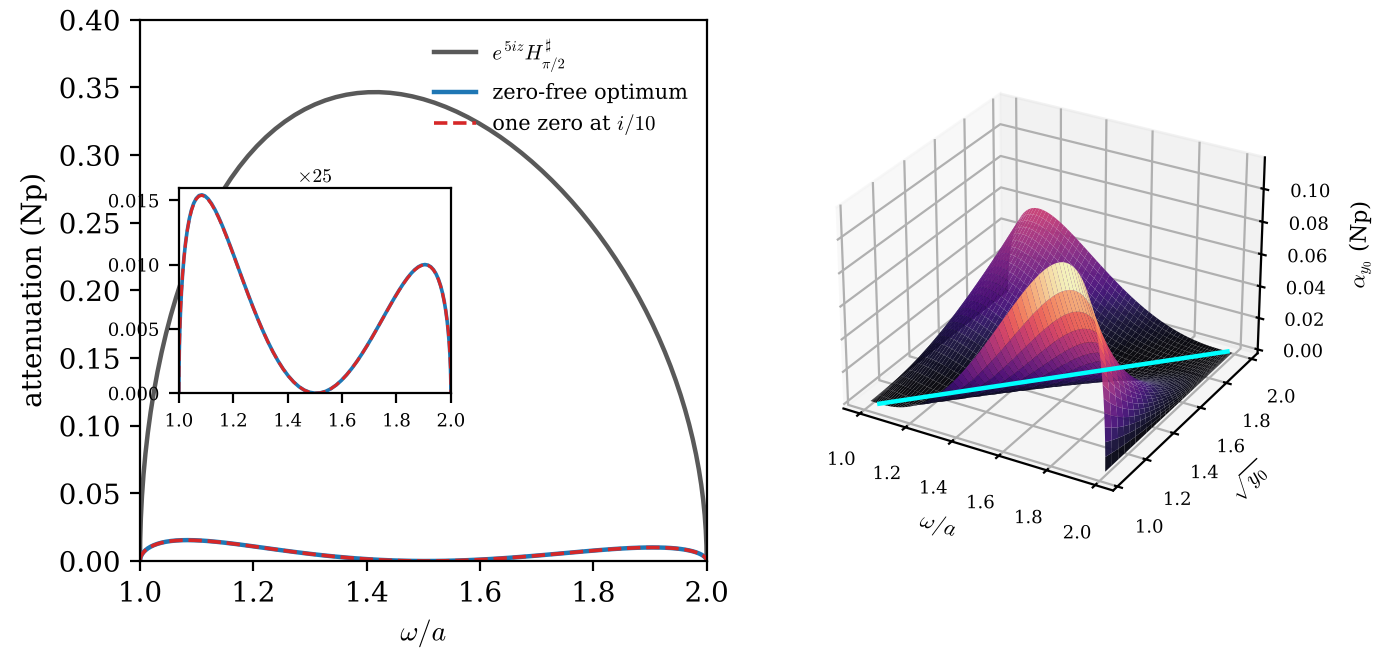
\includegraphics[width=0.8\textwidth]{figures/fig_delay.png}
\caption{The argument $\pi/2+5\omega$ on an octave. Left: the attenuation of
the delayed optimum $e^{5iz}\Hs_{\pi/2}$ (\cref{thm:allzeros}), of the zero-free
optimum of \cref{thm:exactmean}, which touches zero at $x_*=1.5049$, and of
the system with one zero of \cref{prop:onezerodelay}. Right: the zero-free
systems $H_{y_0}$ of \cref{thm:delay}, each lossless at a different
frequency $\sqrt{y_0}$.}
\label{fig:delay}
\end{figure*}

\begin{figure}[t]
\centering
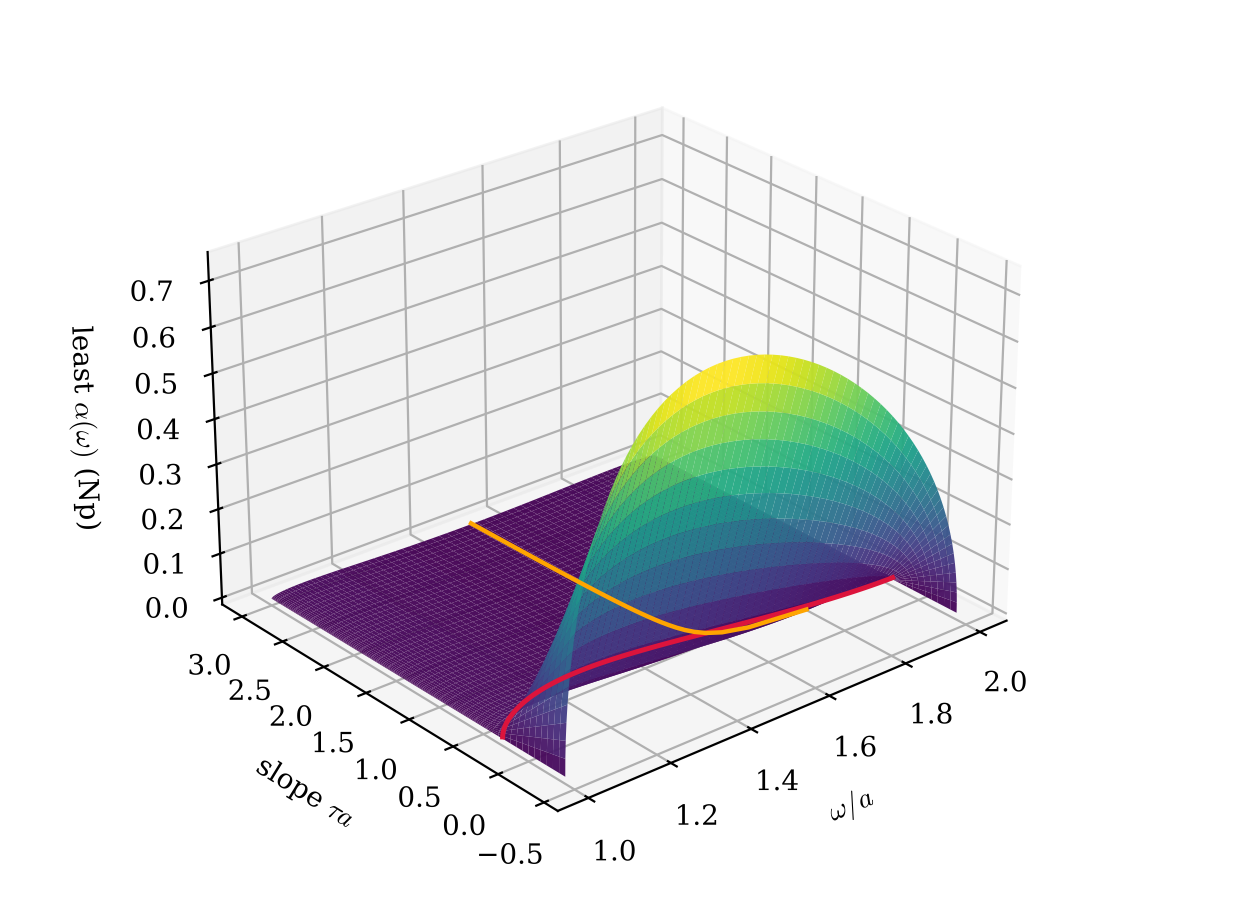
\includegraphics[width=\columnwidth]{figures/fig_exactmean.png}
\caption{The least attenuation of \cref{thm:exactmean} on an octave for the
phase $-1+\tau\omega$, as a function of $\tau$. Up to $\tau_c=0.2852$ it is
pointwise optimal and decreases linearly in $\tau$; beyond it the
resonance above the band moves in from infinity and the profile touches
zero at the contact $x_*$.}
\label{fig:exactmean}
\end{figure}

\subsection{A delay together with zeros}\label{ssec:delayzeros}

\Cref{lem:zeroatom} shows how a zero enters. A zero at $i\varepsilon$ adds
$p_\varepsilon(t)=2\arctan(\varepsilon/t)=2\int_0^\varepsilon j_u(t)\dd u$ to the
phase that the zero-free factor must carry, since $\arg(-B_\varepsilon)=\pi-p_\varepsilon$
on the real axis; and $p_\varepsilon$ costs, in the bound
\eqref{eq:globallower}, what a measure at the negative squared frequencies
$-u^2$ would cost.

\begin{proposition}\label{prop:onezerodelay}
On $[1,2]$, for the argument $\pi/2+5\omega$, there is a passive system with
one zero, at $i/10$, whose mean attenuation is less than
$\mathcal M_{\pi/2}(5)$. So the least zero-free mean is not the least mean
with zeros allowed.
\end{proposition}

\begin{proof}
Let $s=\pi/2$, $\varepsilon=1/10$, $g_0=-s+5t$ and
$g_\varepsilon=g_0+p_\varepsilon$. By \cref{lem:zeroatom},
\begin{gather*}
-\frac{x\,v_{g_\varepsilon}(x)}{r(x)}=q_\varepsilon(x^2),\qquad
q_\varepsilon=sq-P,\\
P(y)=2\int_0^\varepsilon\frac{y\dd u}{(y+u^2)Q_u},\\
\beta_{g_\varepsilon}=5-s\tau_\circ+2\int_0^\varepsilon\frac{\dd u}{Q_u}>0.
\end{gather*}
On $[1,4]$, the integrands of \cref{thm:delay} are at least $1/64$ and $1/512$,
and $\tau_\circ\ge1/2$, as $K(k)\ge\pi/2$, so $q'\ge1/128$ and $-q''\ge1/1024$; and $0\le P'\le
\varepsilon^3/3$, $0\le-P''\le2\varepsilon^3/3$. Hence $q_\varepsilon'>0$ and
$q_\varepsilon''<0$ there. For $\frac94\le y\le4$ the same integral gives
$q-yq'\ge3/32$, and $P\le\varepsilon$, so $q_\varepsilon-yq_\varepsilon'\ge
\frac{3\pi}{64}-\frac1{10}>0$; also $q_\varepsilon(4)\ge\frac\pi8-\varepsilon>0$, since
$q(4)\ge\tau_\circ/2$. The proof of \cref{thm:exactmean}(ii), with $sq$ replaced by
$q_\varepsilon$ and $\tau-s\tau_\circ$ by $\beta_{g_\varepsilon}>-q_\varepsilon(4)$, gives $v>4$ and $C,D>0$ with
$x_*=x(v)\in(\frac32,2)$, and the Herglotz function
$h_\varepsilon=h_{g_\varepsilon}+R(C/z+Dz/(v-z^2))$ with linear coefficient $0$.
The system $H_\varepsilon=-B_\varepsilon e^{ih_\varepsilon}$ is passive, has one zero, at
$i\varepsilon$, and $\arg H_\varepsilon=\pi-p_\varepsilon+g_\varepsilon=\pi/2+5\omega$ on the
band.

For a phase $g$ and this $x_*$, let
$\mathcal L(g)=\int_a^bv_g-\lambda_1x_*v_g(x_*)/r(x_*)-\lambda_2\beta_g$. The
proof of \eqref{eq:globallower} shows that $\int_a^b\alpha\ge\mathcal L(g)$
for every zero-free admissible system with phase $g$, with equality for
$h_\varepsilon$. By \cref{lem:zeroatom},
\[
\mathcal L(j_u)=\frac1{Q_u}\Big(\Gamma_-(-u^2)-\lambda_1\frac{y_*}{y_*+u^2}-\lambda_2\Big),
\]
For $w<0$ put $x(w)=(w+\sqrt{(a^2-w)(b^2-w)}+ab)/(a+b)$, which lies in
$(ab/f,f)$, and $\rho=x(w)-f\in(-\ell^2/f,0)$. Then again
$w=f^2+\ell^2+f(\rho+\ell^2/\rho)$, and $\pi f\rho=-\Gamma_-(w)$. The identity
\eqref{eq:square} is a polynomial identity in $\rho$ and $\varepsilon$, so with
$\Gamma_+(w)$ replaced by $-\Gamma_-(w)$ it reads
\begin{multline*}
(y_*-w)\Big(\Gamma_-(w)-\lambda_1\frac{y_*}{y_*-w}-\lambda_2\Big)\\
=\pi f\Big(f+\frac{\ell^2}\rho\Big)(\rho-x_*+f)^2<0,
\end{multline*}
because $f+\ell^2/\rho<0$. With $w=-u^2$ this gives $\mathcal L(j_u)<0$, so
$\mathcal L(p_\varepsilon)=2\int_0^\varepsilon\mathcal L(j_u)\dd u<0$. The Blaschke
factor has modulus $1$ on $\R$, and
\[
\int_1^2\alpha_{H_\varepsilon}=\mathcal L(g_0)+\mathcal L(p_\varepsilon)
<\mathcal L(g_0)\le\mathcal M_{\pi/2}(5),
\]
the last step by \eqref{eq:globallower} for $g_0$.
\end{proof}

The mean of $H_{1/10}$ is
\[
-s\Lambda+2\int_0^{1/10}\frac{\Gamma_-(-u^2)}{Q_u}\dd u+C\,\Gamma_0+D\,\Gamma_+(v)
=0.0063752
\]
nepers, against $\mathcal M_{\pi/2}(5)=0.0063903$.

\begin{remark}[computed, not proved]\label{rem:onezerofamily}
The construction of \cref{prop:onezerodelay} works for every height
$\varepsilon$ of the zero up to $\varepsilon_0=0.47247$, where the origin
coefficient $C$ vanishes, and the mean then decreases to $0.0051493$ nepers.
With a pair of zeros at $\pm1.3654+1.2608i$ instead, a linear program for
the measure off the band, with the positivity of the attenuation imposed at
$399$ points of the band, gives about $4.3\times10^{-4}$ nepers; without zeros
the same program gives $0.00658$ in place of $0.0063903$, so it is accurate to
a few per cent. These numbers come from computations only. \Cref{prop:sixtap} below proves a mean less than
$7\times10^{-4}$ with six taps.
\end{remark}

\emph{The optimum exists.} The admissible systems are not a convex set, but
a weaker class is. For a measurable $\psi$ on $[a,b]$ let $\mathcal P_\psi$ be
the set of passive systems $H$ with $e^{-i\psi}H\ge0$ almost everywhere on
$[a,b]$, and put
\[
J(H)=\int_a^b-\log\abs{H(\omega)}\dd\omega\in[0,\infty] .
\]
Systems in $\mathcal P_\psi$ may have zeros and need not be regular on the
band. Every system admissible for $\theta$ lies in $\mathcal P_\theta$, and the
systems of \cref{prop:onezerodelay,thm:poisson,thm:expdecay} lie in
$\mathcal P_{\theta+\tau\omega}$.

\begin{theorem}\label{thm:convex}
Let $\psi$ be measurable on $[a,b]$, and suppose that $J(G)<\infty$ for some
$G\in\mathcal P_\psi$.
\begin{enumerate}
\item[(i)] There is exactly one $H_\psi\in\mathcal P_\psi$ with
$J(H_\psi)=\inf_{\mathcal P_\psi}J$.
\item[(ii)] An $H\in\mathcal P_\psi$ with $J(H)<\infty$ is $H_\psi$ if and only if
\[
\int_a^b\frac{\abs{G}}{\abs H}\dd\omega\le b-a\qquad\text{for every }G\in\mathcal P_\psi .
\]
\item[(iii)] Every $G\in\mathcal P_\psi$ satisfies
$\int_a^b\abs{G-H_\psi}^2\dd\omega\le2\big(J(G)-J(H_\psi)\big)$.
\item[(iv)] For $z\in\Cp$ let $P_z(t)=\Im z/(\pi\abs{t-z}^2)$,
$\omega_z=\int_SP_z$ and $M_z=\max_SP_z$, with $S=[-b,-a]\cup[a,b]$. Then
\[
\abs{G(z)-H_\psi(z)}\le2^{1-\omega_z}\Big(\frac{4M_z}{\omega_z}\big(J(G)-J(H_\psi)\big)\Big)^{\omega_z/2}.
\]
\end{enumerate}
\end{theorem}

\begin{proof}
The conditions $\abs H\le1$, $H(-\bar z)=\overline{H(z)}$ and $e^{-i\psi}H\ge0$
almost everywhere are kept by convex combinations, so $\mathcal P_\psi$ is
convex. On $\mathcal P_\psi$, $J(H)=\int_a^b-\log(e^{-i\psi}H)$, and $-\log$ is
convex on $[0,\infty)$, so $J$ is convex.

(i) Let $J_*$ be the infimum and $J(H_k)\to J_*$. The boundary functions are
bounded by $1$ in $L^\infty(\R)$, so a subsequence converges weak-$*$ to some
$\phi$. Since $H_k$ is the Poisson integral of its boundary function
\cite[Ch.~I]{garnett}, $H_k(z)\to H(z)$, the Poisson integral of $\phi$, at
every $z\in\Cp$; so $H$ is analytic, $\abs H\le1$, $H(-\bar z)=\overline{H(z)}$,
and $H=\phi$ almost everywhere on $\R$. On $(a,b)$ the boundary functions
converge weakly in $L^2$, so by Mazur's lemma there are convex combinations
$G_k$ of $H_k,H_{k+1},\dots$ with $G_k\to H$ in $L^2(a,b)$, and almost
everywhere along a subsequence. Each $G_k$ lies in $\mathcal P_\psi$, and
$J(G_k)\le\sup_{j\ge k}J(H_j)\to J_*$ by convexity. The limit of the
nonnegative functions $e^{-i\psi}G_k$ is nonnegative, so $H\in\mathcal P_\psi$,
and Fatou's lemma, with $-\log\ge0$ on $[0,1]$ and lower semicontinuous, gives
$J(H)\le J_*$. If $H$ and $H'$ are both minimisers, then $J_*<\infty$, and
$J(\frac12(H+H'))<J_*$ unless $\abs H=\abs{H'}$ almost everywhere on $(a,b)$,
by strict convexity of $-\log$. Then $H=H'$ almost everywhere on $(a,b)$, since
both have argument $\psi$ where they do not vanish, and $H=H'$ by the
boundary uniqueness theorem \cite[Ch.~II]{garnett}.

(ii) Here $H\ne0$ almost everywhere on $(a,b)$. Put $\rho=\abs G/\abs H$. If the
inequality holds, then $-\log\abs G\ge-\log\abs H-(\rho-1)$, and integrating
gives $J(G)\ge J(H)+(b-a)-\int\rho\ge J(H)$. Conversely, let $H=H_\psi$ and
$0<t\le\frac12$. Then $H_t=(1-t)H+tG\in\mathcal P_\psi$ and
$\abs{H_t}=\abs H(1+t(\rho-1))$, so
\[
0\le\frac{J(H_t)-J(H)}t=\int_a^b\frac{-\log\big(1+t(\rho-1)\big)}t\dd\omega .
\]
The integrand is a difference quotient of a convex function of $t$, so it
decreases as $t\downarrow0$, to $1-\rho$, and it is at most $2\log2$ at
$t=\frac12$. By monotone convergence $\int(1-\rho)\ge0$.

(iii) We may take $J(G)<\infty$. Put $\rho_0=e^{-i\psi}H_\psi$ and
$\rho_1=e^{-i\psi}G$, which lie in $(0,1]$ almost everywhere. Since $-\log$ has
second derivative at least $1$ on $(0,1]$,
\begin{multline*}
-\log\big((1-t)\rho_0+t\rho_1\big)\\
\le-(1-t)\log\rho_0-t\log\rho_1-\tfrac12t(1-t)(\rho_1-\rho_0)^2 ,
\end{multline*}
and $\abs{\rho_1-\rho_0}=\abs{G-H_\psi}$. Integrating, and using
$J((1-t)H_\psi+tG)\ge J(H_\psi)$, gives
$\frac12(1-t)\int\abs{G-H_\psi}^2\le J(G)-J(H_\psi)$; let $t\to0$.

(iv) Let $D=G-H_\psi\ne0$, so $\abs D\le2$. As $\log\abs D$ is subharmonic and
bounded above, it lies below the Poisson integral of its boundary values;
with Jensen's inequality for the probability density $P_z/\omega_z$ on $S$,
\[
\log\abs{D(z)}\le(1-\omega_z)\log2+\frac{\omega_z}2\log\Big(\frac1{\omega_z}\int_SP_z\abs D^2\Big).
\]
By the symmetry, $\int_S\abs D^2=2\int_a^b\abs D^2$, and (iii) gives the bound.
\end{proof}

For a constant phase the minimiser is the system of \cref{thm:allzeros}. The
proof of \cref{prop:compare} uses the continuity of $F$ only to pass from
almost every point of the band to every point; without it, it shows
$\alpha\ge\as_\theta$ almost everywhere for every nonconstant $H\in\mathcal
P_\theta$. Hence $H_\theta=\Hs_\theta$ for $0<\theta<\pi$, and by
\cref{thm:convex}(ii) every $G\in\mathcal P_\theta$ has
$\int_a^b\abs G/\abs{\Hs_\theta}\le b-a$. For $\psi=\theta+\tau\omega$ with $\tau>0$
we have not found $H_\psi$ in closed form, but it is the limit of explicit
passive polynomials, each of them the solution of a finite convex problem.%
\footnote{Parts (iii) and (iv) of \cref{thm:convex}, \cref{lem:toeplitz,lem:tail,lem:chebnorm},
\cref{thm:construction,thm:regularity,thm:sharperate}, \cref{prop:sixtap,prop:commuting}
and \cref{cor:allbands} were found with OpenAI's Codex, starting from
\cref{thm:convex,thm:expdecay}; the proofs were checked step by step and every
number recomputed (\cref{app:verification}).}

Fix $\sigma>0$ and put $w(z)=(z-i\sigma)/(z+i\sigma)$, which maps $\Cp$ onto the
unit disc $\mathbb D$. A function $f$ on $\mathbb D$ with $\abs f\le1$ gives the
passive system $H=f\circ w$, and $H(-\bar z)=\overline{H(z)}$ exactly when the
Taylor coefficients $c_k$ of $f$ are real. For $c=(c_0,\dots,c_N)$ let
$T_N(c)$ be the lower triangular Toeplitz matrix with entries $c_{i-j}$ for
$i\ge j$, $0\le i,j\le N$.

\begin{lemma}\label{lem:toeplitz}
If $\abs f\le1$ on $\mathbb D$, then $\|T_N(c)\|\le1$ and
$\sum_{k\le N}c_k^2\le1$. Conversely, if $c\in\R^{N+1}$ and $\|T_N(c)\|\le1$,
then $p_N(w)=\sum_{k=0}^N(1-\frac k{N+1})c_kw^k$ satisfies $\abs{p_N}\le1$ on
$\mathbb D$.
\end{lemma}

\begin{proof}
Multiplication by $f$ is a contraction of the Hardy space $H^2(\mathbb D)$, and
$T_N(c)$ is its compression to the polynomials of degree at most $N$; its
first column has squared norm $\sum_{k\le N}c_k^2$. For the converse let
$\abs w=1$ and $u=(1,\bar w,\dots,\bar w^N)^{\mathsf T}$. The entry $c_k$ occurs
$N+1-k$ times on the $k$-th subdiagonal, so $u^*T_N(c)u=(N+1)p_N(w)$, and
$\abs{u^*T_Nu}\le\|T_N\|\,\|u\|^2=N+1$. The maximum principle gives the bound
in $\mathbb D$.
\end{proof}

The condition $\|T_N(c)\|\le1$ is the linear matrix inequality
$\left(\begin{smallmatrix}I&T_N\\T_N^{\mathsf T}&I\end{smallmatrix}\right)\succeq0$,
so every feasible $c$ gives a system $p_N\circ w$ that is passive in all of
$\Cp$, not only at sampled frequencies. The phase enters through moments.
Let $\psi$ be $C^1$ on $[a,b]$, and for an interval $I=[u,v]\subset[a,b]$ put
\begin{gather*}
A_{I,k}=\int_u^ve^{-i\psi(x)}w(x)^k\dd x,\\
C_I=2j(v)+\int_u^vj\,\abs{\psi'},\qquad j(x)=\frac{x^2+\sigma^2}{2\sigma}.
\end{gather*}
If $\abs f\le1$, then $\int_Ie^{-i\psi}H=\sum_kc_kA_{I,k}$, since the boundary
values $\sum c_kw^k$ converge in $L^2$.

\begin{lemma}\label{lem:tail}
$\abs{A_{I,k}}\le C_I/k$ for $k\ge1$, so
$(\sum_{k>N}\abs{A_{I,k}}^2)^{1/2}\le\delta_{N,I}=C_I/\sqrt N$, and for
$\abs f\le1$,
\[
\Big|\int_Ie^{-i\psi}H-\sum_{k=0}^Nc_kA_{I,k}\Big|\le\delta_{N,I} .
\]
\end{lemma}

\begin{proof}
On $(0,\infty)$, $w(x)=e^{it}$ with $t=-2\arctan(\sigma/x)$ and $\dd x/\dd t=j(x)$.
With $\beta(t)=j(x)e^{-i\psi(x)}$, integration by parts in
$A_{I,k}=\int\beta e^{ikt}\dd t$ bounds $k\abs{A_{I,k}}$ by
$j(u)+j(v)+\int_u^v(j'+j\abs{\psi'})=C_I$, as $j'>0$. Then
$\sum_{k>N}k^{-2}\le1/N$, and Cauchy--Schwarz with $\sum c_k^2\le1$ bounds the
tail of the series.
\end{proof}

For an affine phase $\theta+\tau\omega$,
$C_I=(v^2+\sigma^2)/\sigma+\abs\tau\big((v^3-u^3)/(6\sigma)+\sigma(v-u)/2\big)$.
Let $\mathcal D_n$ be the partition of $[a,b]$ into $2^n$ equal intervals, and
let $N_n\to\infty$. The \emph{$n$-th problem} has the unknowns
$c\in\R^{N_n+1}$ and $r_I\ge0$ for $I\in\mathcal D_n$; for a coarser dyadic
interval $r_I$ is the sum over the intervals of $\mathcal D_n$ in it. It asks
for
\begin{gather*}
\|T_{N_n}(c)\|\le1,\qquad0\le r_I\le\abs I\quad(I\in\mathcal D_n),\\
\Big|\sum_{k\le N_n}c_kA_{I,k}-r_I\Big|\le\delta_{N_n,I}\quad(I\in\mathcal D_0\cup\dots\cup\mathcal D_n),
\end{gather*}
and minimises $V_n=\sum_{I\in\mathcal D_n}\abs I\,(-\log(r_I/\abs I))$. Its least
value is $v_n$. The constraints are a matrix inequality and second-order
cones, and the objective is convex.

\begin{theorem}\label{thm:construction}
Let $\psi$ be $C^1$ on $[a,b]$ and suppose that $J(G)<\infty$ for some
$G\in\mathcal P_\psi$.
\begin{enumerate}
\item[(i)] Each $n$-th problem has a minimiser, and $0\le v_n\le J(H_\psi)$.
\item[(ii)] $v_n\to J(H_\psi)$.
\item[(iii)] If $(c^{(n)},r^{(n)})$ is feasible with $V_n\le v_n+\varepsilon_n$
and $\varepsilon_n\to0$, then the passive systems
\[
H_n(z)=\sum_{k=0}^{N_n}\Big(1-\frac k{N_n+1}\Big)c^{(n)}_k\Big(\frac{z-i\sigma}{z+i\sigma}\Big)^k
\]
converge to $H_\psi$ locally uniformly in $\Cp$.
\end{enumerate}
\end{theorem}

\begin{proof}
(i) For $H\in\mathcal P_\psi$ with $J(H)<\infty$, its first $N_n+1$
coefficients and $r_I=\int_I\abs H=\int_Ie^{-i\psi}H$ are feasible by
\cref{lem:toeplitz,lem:tail}, and Jensen's inequality on each interval gives
$V_n\le J(H)$. Taking $H=H_\psi$, $v_n\le J(H_\psi)$. The feasible set is compact
and $V_n$ is lower semicontinuous, so a minimiser exists.

(ii), (iii) The $H_n$ are passive by \cref{lem:toeplitz}. By Montel's theorem a
subsequence converges locally uniformly to some $H$ with $\abs H\le1$, with
coefficients $c_k$; then $c^{(n)}_k\to c_k$ for each $k$, and
$\sum_kc_k^2\le1$. For a fixed dyadic interval $I$, $(A_{I,k})_k$ is square
summable, so splitting the sums at a fixed $K$ gives
$\sum_{k\le N_n}c^{(n)}_kA_{I,k}\to\sum_kc_kA_{I,k}=\int_Ie^{-i\psi}H$; as
$\delta_{N_n,I}\to0$, $r^{(n)}_I\to\int_Ie^{-i\psi}H$, which therefore lies in
$[0,\abs I]$. By the dyadic differentiation theorem $e^{-i\psi}H\ge0$ almost
everywhere, and $H\in\mathcal P_\psi$. For a fixed level $q\le n$, convexity of
$-\log$ gives $V_n\ge\Phi_q^{(n)}=\sum_{I\in\mathcal D_q}\abs I(-\log(r^{(n)}_I/\abs I))$,
and in the limit
\[
\liminf_nV_n\ge\Phi_q(H)=\sum_{I\in\mathcal D_q}\abs I\Big(-\log\frac1{\abs I}\int_I\abs H\Big).
\]
By Jensen's inequality $\Phi_q(H)$ increases with $q$ and is at most $J(H)$;
the averages of $\abs H$ converge to $\abs H$ almost everywhere, so Fatou's
lemma gives $\Phi_q(H)\to J(H)$. Hence
$J(H_\psi)\le J(H)\le\liminf V_n\le\liminf(v_n+\varepsilon_n)\le J(H_\psi)$. So
$H=H_\psi$ by \cref{thm:convex}(i), the limit does not depend on the
subsequence, and $v_n\to J(H_\psi)$.
\end{proof}

The finite problems carry the phase only through the moments, so the $H_n$
do not have the phase $\psi$ exactly; it is attained in the limit.
\Cref{thm:construction} gives neither a closed form for $H_\psi$ nor a rate
for $v_n\to J(H_\psi)$. For an analytic phase the optimum has no zeros inside
the band.

\begin{theorem}\label{thm:regularity}
Let $\psi$ be real analytic on $(a,b)$, and suppose that some
$G\in\mathcal P_\psi$ with $J(G)<\infty$ is continuous and nonzero on $(a,b)$.
Then $H_\psi$ extends analytically across $(a,b)$, has no zeros there, and
its attenuation is real analytic on $(a,b)$.
\end{theorem}

\begin{proof}
Near $x_0\in(a,b)$, $F=e^{-i\psi}H_\psi$ is bounded and analytic on the upper
side, and its boundary values are real almost everywhere. Its imaginary part
is a bounded harmonic function, hence the Poisson integral of its boundary
values, which vanish on the interval; so it is continuous up to the
interval with value $0$, and the Schwarz reflection principle continues $F$
across it. On the interval $F\ge0$, and $F\not\equiv0$ because
$J(H_\psi)<\infty$, so a zero at $x_0$ has even order $2k\ge2$ and
$\abs{H_\psi(x)}\le C\abs{x-x_0}^{2k}$ nearby. As $\abs G\ge c>0$ near $x_0$,
$\abs G/\abs{H_\psi}$ is not integrable, against \cref{thm:convex}(ii).
\end{proof}

For every $\psi\in C^1[a,b]$ such a $G$ exists: by \cref{thm:multiband}, with one
band and $n=1$, there is a zero-free passive system with phase $\psi$,
continuous and nonzero on $[a,b]$. So the hypotheses of
\cref{thm:convex,thm:construction} hold for every such phase, and for an
affine phase $H_{\theta+\tau\omega}$ is analytic and has no zeros inside the band,
though it may have zeros in $\Cp$; whether it is continuous at $a$ and $b$ is
not known. The rest of this subsection shows how small its loss is.

There is still a positive floor. For $y>0$ let $P_y(x)=y/(\pi(x^2+y^2))$ and
$\omega_y=\int_a^bP_y$.

\begin{theorem}\label{thm:poisson}
Let $\theta\notin\pi\Z$, $\tau\ge0$ and $H\in\mathcal P_{\theta+\tau\omega}$.
For every $y>0$,
\begin{gather*}
\frac1{b-a}\int_a^b\alpha\ \ge\ \frac{\omega_y}{(b-a)P_y(a)}\,\log\frac1{1-\varepsilon_y}>0,\\
\varepsilon_y=\Big(\frac{\abs{\sin\theta}\,e^{-\tau y}}{2^{1-\omega_y}}\Big)^{1/\omega_y}\in(0,1).
\end{gather*}
\end{theorem}

\begin{proof}
Let $J=H-e^{i\theta+i\tau z}$, analytic in $\Cp$ with $\abs J\le2$. On the
imaginary axis $H(iy)$ is real, so
$\abs{J(iy)}\ge\abs{\sin\theta}e^{-\tau y}>0$. Almost everywhere on the band
$\abs{J(x)}=1-e^{-\alpha(x)}$. As $\log\abs J$ is subharmonic and bounded
above, it lies below the Poisson integral of its boundary values
\cite[Ch.~II]{garnett}, so
\[
\log\big(\abs{\sin\theta}e^{-\tau y}\big)\le\int_a^bP_y\log\big(1-e^{-\alpha}\big)
+(1-\omega_y)\log2 .
\]
Since $u\mapsto\log(1-e^{-u})$ is increasing and concave, Jensen's
inequality for the probability density $P_y/\omega_y$ on $[a,b]$ gives
$\omega_y^{-1}\int_a^bP_y\alpha\ge\log(1/(1-\varepsilon_y))$, and $P_y\le P_y(a)$
on the band.
\end{proof}

The floor is exponentially small in $\tau$, and so is the loss that zeros
make possible. Let $\tau_\circ$ be as in \cref{lem:q}.

\begin{theorem}\label{thm:expdecay}
Let $\theta\in\R$ and $a\tau\ge12$. There is a passive system $H$, regular on the
band, with $\arg H\equiv\theta+\tau\omega$ on $[a,b]$ and
\[
\frac1{b-a}\int_a^b\alpha\le e^{3-a\tau/e}\Big(2+\frac\pi4(b-a)\tau_\circ
+\frac{b(b^2-a^2)}{2e\,a^2}\,\tau\Big).
\]
\end{theorem}

The idea is to turn $\cos\theta+i\sin\theta$ into a function that is close to
$e^{i\theta}$ on the band and is cancelled by the delay $e^{i\tau z}$ in the upper
half-plane: a smoothed sign function of exponential type $\tau$.

\begin{proof}
\emph{The kernel.} Let $m=2\lfloor a\tau/(2e)\rfloor$, so that $m$ is even,
$4\le m\le a\tau/e$ and $m>a\tau/e-2$, and let $\kappa=\tau/m\ge e/a$. Put
\begin{gather*}
I_m=\int_\R\Big(\frac{\sin u}u\Big)^m\dd u,\qquad
T(z)=2\int_0^zK,\\
K(\zeta)=\frac\kappa{I_m}\Big(\frac{\sin\kappa\zeta}{\kappa\zeta}\Big)^m .
\end{gather*}
$K$ is entire, even, nonnegative on $\R$, with $\int_\R K=1$. So $T$ is entire,
odd, real and increasing on $\R$, with $\abs T\le1$ there. Since
$\sin w/w=\int_0^1\cos(tw)\dd t$, $\abs{\sin w/w}\le e^{\abs{\Im w}}$, so
$\abs{K(x+iy)}\le(\kappa/I_m)e^{\tau\abs y}$ and
$\abs{T(x+iy)}\le1+2\kappa e^{\tau\abs y}/(\tau I_m)$.

\emph{The factor $F$.} Let $S=\cos\theta+i\sin\theta\,T$ and $F=e^{i\tau z}S$.
By the last bound $F$ is bounded in $\Cp$; it is continuous up to $\R$ and
$\abs{F(x)}^2=\cos^2\theta+\sin^2\theta\,T(x)^2\le1$ there. So $F$ is the
Poisson integral of its boundary values and $\abs F\le1$ in $\Cp$. As $T$ has
real coefficients and is odd, $F(-\bar z)=\overline{F(z)}$.

\emph{The band.} For $x\ge a$,
\[
0\le1-T(x)=2\int_x^\infty K\le\frac{2(\kappa x)^{1-m}}{(m-1)I_m}\le\varepsilon
=\frac{2(\kappa a)^{1-m}}{(m-1)I_m},
\]
and $0\le T'(x)=2K(x)\le(m-1)\varepsilon/a$. Since $\sin u/u\ge1-u^2/6\ge0$ for
$\abs u\le\sqrt6$ and $(1-v^2)^m\ge1-mv^2$,
\begin{align*}
I_m&\ge\sqrt6\int_{-1}^1(1-v^2)^m\dd v\\
&\ge\sqrt6\int_{\abs v\le m^{-1/2}}(1-mv^2)\dd v
=\frac{4\sqrt6}{3\sqrt m}>\frac3{\sqrt m} .
\end{align*}
With $2\sqrt m\le3(m-1)$, $\kappa a\ge e$ and $m>a\tau/e-2$, this gives
$\varepsilon\le(\kappa a)^{1-m}\le e^{3-a\tau/e}$, and $\varepsilon\le e^{3-12/e}<\frac14$.
On $[a,b]$, $T\in[1-\varepsilon,1]$, so $\abs S\ge1-\varepsilon$ and
$-\log\abs S\le-\log(1-\varepsilon)\le2\varepsilon$. Write
$\arg S=\theta+\delta$ there, with $\delta$ continuous. The derivative of
$\arg(\cos\theta+i\sin\theta\,T)$ in $T$ is
$\sin\theta\cos\theta/(\cos^2\theta+\sin^2\theta\,T^2)$, at most
$\frac12(1-\varepsilon)^{-2}\le\frac89$ in modulus, so $\abs\delta\le\varepsilon$ and
$\abs{\delta'}\le T'\le(m-1)\varepsilon/a$.

\emph{The phase correction.} Let $g=-\delta$ and $G(t)=g(t)/t$ on $[a,b]$. Then
$\abs{G'}\le\abs{\delta'}/a+\abs\delta/a^2\le m\varepsilon/a^2$. By Glauert's
integral (proof of \cref{lem:q}), the function $v_g$ of \cref{prop:profile} is
\[
v_g(x)=\frac{2x\,r(x)}\pi\int_a^b\frac{t\,(G(t)-G(x))}{r(t)\,(x^2-t^2)}\dd t,
\]
and here $\abs{G(t)-G(x)}\le\abs{x^2-t^2}\max\abs{G'}/(2a)$, while
$\int_a^bt\dd t/r(t)=\pi/2$ and $x\,r(x)\le b(b^2-a^2)/2$. So
\[
\abs{v_g}\le\eta=\frac{b(b^2-a^2)\,m\,\varepsilon}{4a^3}
\le\frac{b(b^2-a^2)\,\tau\,\varepsilon}{4e\,a^2} .
\]
Also $\abs{\beta_g}\le\tau_\circ\varepsilon$. Put $c=\max(0,-\beta_g)$ and
$h=h_g+cR/z$. As in the proof of \cref{prop:profile}(iii), $\Im(h_g-\beta_gz)$
is harmonic in $\Cp$, continuous up to $\R$, zero on $\R\setminus S$, equal to
$v_g\ge-\eta$ on the band, and tends to $0$ at infinity, so
$\Im h_g\ge\beta_g\Im z-\eta$. By \cref{lem:R}, $R(0)=-ab$, $R$ is even and
$R(z)=z^2+O(1)$, so $(R+ab)/z-z$ is analytic in $\C\setminus S$, real on
$\R\setminus S$, $O(z^{-1})$ at infinity, and has imaginary part $r(x)/x\ge0$
on the upper side of the band; hence its imaginary part is nonnegative in
$\Cp$, and $\Im(R/z)\ge\Im z+ab\Im(-1/z)\ge\Im z$. So
\[
\Im h\ge(\beta_g+c)\Im z-\eta\ge-\eta\qquad\text{in }\Cp .
\]

\emph{The system.} Let $H=e^{-\eta}F\,e^{ih}$. Then $\abs H\le1$ in $\Cp$, and
$H(-\bar z)=\overline{H(z)}$ because $h$ is odd and real on $\R\setminus S$. It
is continuous up to an open interval around $[a,b]$ and has no zeros there.
On the band $\Re h=g=-\delta$, so $\arg H=\tau\omega+\theta+\delta-\delta=\theta+\tau\omega$,
and
\[
\alpha=\eta-\log\abs S+v_g+c\,\frac rx .
\]
With $\int_a^br/x=\frac\pi4(b-a)^2$ the mean is at most
$2\eta+2\varepsilon+\frac\pi4(b-a)\tau_\circ\varepsilon$, which is the bound.
\end{proof}

For $\theta=\pi/2$ the factor $S=iT$ already has the exact argument $\pi/2$, so
$h=0$, $\eta=0$ and $\alpha=-\log T$. On the octave its mean is
$1.7\times10^{-3}$ nepers at $\tau=12$, $4.9\times10^{-5}$ at $\tau=20$ and
$1.4\times10^{-7}$ at $\tau=30$, against the zero-free floor $0.0060483$ of
\cref{prop:floor}.

A polynomial kernel in $\sin dz$ in place of the sinc power gives a larger
exponent. Approximating the sign by polynomials and entire functions is
classical \cite{eremenkoyuditskii}, as are linear-phase filters with finitely
many taps \cite{parksmcclellan}; we need only the explicit kernel below, whose
passivity is checked directly. Put
\begin{gather*}
d=\frac\pi{a+b},\qquad s_0=\sin da,\qquad \gamma=\operatorname{artanh}s_0,\\
C_{a,b}=\frac\gamma d=\frac{a+b}\pi\log\cot\frac{\pi(b-a)}{4(a+b)} .
\end{gather*}
As $\operatorname{artanh}(\sin t)=\int_0^t\sec u\dd u>t$ for $0<t<\pi/2$,
$C_{a,b}>a$. With the Chebyshev polynomial $T_m$, $T_m(\cos t)=\cos mt$, let
\begin{gather*}
K_m(s)=T_m\Big(\frac{2s^2-1-s_0^2}{1-s_0^2}\Big)^2,\\
\mathcal I_m=\int_0^1K_m,\qquad \Pi_m(s)=\frac1{\mathcal I_m}\int_0^sK_m .
\end{gather*}
$\Pi_m$ is an odd polynomial of degree $4m+1$, increasing on $[-1,1]$ from $-1$
to $1$. For $s_0\le s\le1$ the argument of $T_m$ lies in $[-1,1]$, so
$K_m(s)\le1$ and $0\le1-\Pi_m(s)\le\epsilon_m=(1-s_0)/\mathcal I_m$. On $[a,b]$,
$\sin d\omega\in[s_0,1]$, so $U_m(\omega)=\Pi_m(\sin d\omega)$ satisfies
$1-\epsilon_m\le U_m\le1$ and $\abs{U_m'}\le d/\mathcal I_m$ there.

\begin{lemma}\label{lem:chebnorm}
For $\tau\ge(4m+1)d$ the function
$F_m(z)=e^{i\tau z}(\cos\theta+i\sin\theta\,\Pi_m(\sin dz))$ is passive, and
$\log\mathcal I_m/m\to4\gamma$ as $m\to\infty$.
\end{lemma}

\begin{proof}
Put $q=e^{idz}$ and $N=4m+1$. As $\Pi_m$ is odd with real coefficients,
$q^N(\cos\theta+i\sin\theta\,\Pi_m((q-q^{-1})/(2i)))$ is a polynomial in $q$
with real coefficients. On $\abs q=1$ its modulus is at most $1$, since
$\abs{\Pi_m}\le1$ on $[-1,1]$, so it is at most $1$ for $\abs q\le1$, that is,
in $\Cp$; and $e^{i(\tau-Nd)z}$ is a delay. For $0\le s<s_0$ put
$\chi(s)=\operatorname{arcosh}((1+s_0^2-2s^2)/(1-s_0^2))$, decreasing, with
$\chi(0)=2\gamma$ since $\cosh2\gamma=(1+s_0^2)/(1-s_0^2)$. There
$K_m=\cosh^2(m\chi)$, so $K_m\le e^{4m\gamma}$ on $[0,1]$ and
$\mathcal I_m\le e^{4m\gamma}$; and for $0<h<s_0$,
$\mathcal I_m\ge\int_0^h\frac14e^{2m\chi}\ge\frac h4e^{2m\chi(h)}$. Let
$m\to\infty$ and then $h\to0$.
\end{proof}

\begin{theorem}\label{thm:sharperate}
Let $\theta\in\R$, $m\ge1$, $\tau\ge(4m+1)d$ and $\epsilon_m\le\frac14$. There
is a passive system, regular on the band, with $\arg H\equiv\theta+\tau\omega$ on
$[a,b]$ and
\[
\frac1{b-a}\int_a^b\alpha\le\frac1{\mathcal I_m}\Big(2D_{a,b}+\big(2+\tfrac\pi4(b-a)\tau_\circ\big)(1-s_0)\Big),
\]
where $D_{a,b}=\frac{b(b^2-a^2)}{4a}\big(\frac da+\frac{1-s_0}{a^2}\big)$. For
$\theta=\pi/2$ the system $F_m$ itself has the phase, with mean at most
$2\epsilon_m$.
\end{theorem}

\begin{proof}
Let $S=\cos\theta+i\sin\theta\,U_m$, so that $F_m=e^{i\tau z}S$ is passive by
\cref{lem:chebnorm}. On the band $\abs S\ge1-\epsilon_m$, so
$-\log\abs S\le2\epsilon_m$, and, by the derivative bound in the proof of
\cref{thm:expdecay}, $\arg S=\theta+\delta$ with $\abs\delta\le\epsilon_m$ and
$\abs{\delta'}\le\abs{U_m'}\le d/\mathcal I_m$. The phase correction and the
system are then built as in that proof: with $g=-\delta$ and $G=g/t$,
$\abs{G'}\le\abs{\delta'}/a+\abs\delta/a^2\le(d/a+(1-s_0)/a^2)/\mathcal I_m$, so
Glauert's integral gives $\abs{v_g}\le\eta=D_{a,b}/\mathcal I_m$, and
$\abs{\beta_g}\le\tau_\circ\epsilon_m$. The mean of $e^{-\eta}F_me^{ih}$ is at most
$2\eta+2\epsilon_m+\frac\pi4(b-a)\tau_\circ\epsilon_m$. For $\theta=\pi/2$,
$F_m=ie^{i\tau z}U_m$, $U_m>0$ on the band, and $-\log U_m\le2\epsilon_m$.
\end{proof}

With $m=\lfloor(\tau/d-1)/4\rfloor$, \cref{lem:chebnorm} turns this bound into
$e^{-(C_{a,b}+o(1))\tau}$. On the octave $d=\pi/3$, $s_0=\sqrt3/2$,
$\gamma=\log(2+\sqrt3)$ and
\[
C_{1,2}=\frac3\pi\log(2+\sqrt3)=1.2576021548\ldots,
\]
against $1/e$ from \cref{thm:expdecay}. For the octave, $\Pi_1(s)$ is the
polynomial $P$ below, since $8s^2-7=(2s^2-1-s_0^2)/(1-s_0^2)$; taking $d=1$ in
place of $\pi/3$ lowers the delay $(4m+1)d$ to $5$, at the price of a band
image $[\sin1,1]$ slightly larger than $[s_0,1]$.

\begin{proposition}\label{prop:sixtap}
On $[1,2]$, the passive system
\begin{multline*}
H(z)=\frac1{734}\big(-12-80e^{2iz}-435e^{4iz}\\
+435e^{6iz}+80e^{8iz}+12e^{10iz}\big)
\end{multline*}
has the argument $\pi/2+5\omega$ on the band, no zeros on the band, and
\[
\int_1^2\alpha<\frac7{10000} .
\]
\end{proposition}

\begin{proof}
Let $P(s)=(192s^5-560s^3+735s)/367$. From $\sin3x=3\sin x-4\sin^3x$ and
$\sin5x=16\sin^5x-20\sin^3x+5\sin x$,
$367P(\sin x)=435\sin x+80\sin3x+12\sin5x$, so $H=ie^{5iz}P(\sin z)$. Now
$P(\pm1)=\pm1$ and $P'(s)=\frac{15}{367}(8s^2-7)^2\ge0$, so $\abs P\le1$ on
$[-1,1]$, and $H$ is passive as in \cref{lem:chebnorm}, with $d=1$ and degree
$5$. On $[1,2]$, $\sin x\ge\sin1$, as $\sin$ is concave there and
$\sin2=\sin(\pi-2)>\sin1$, and $\sin1>1-\frac16+\frac1{120}-\frac1{5040}>\frac56$, so
\[
1\ge P(\sin x)>P(\tfrac56)=\frac{59225}{59454}=M,
\]
which gives the argument and the absence of zeros, and $-\log P\le(1-P)/M$.
With $F(t)=t+\frac{176}{1101}t^3+\frac{192}{1835}t^5$ one has
$\frac{\dd}{\dd x}\big(-F(\cos x)\big)=P(\sin x)$, so
$\int_1^2P(\sin x)\dd x=F(\cos1)-F(\cos2)$. The partial sums
$L=\sum_{k=0}^{11}(-1)^k/(2k)!$ and $U=\sum_{k=0}^{12}(-1)^k4^k/(2k)!$ of the
alternating cosine series satisfy $L<\cos1$ and $\cos2<U$, and $F$ is
increasing, so
\[
\int_1^2\alpha\le\frac{1-F(L)+F(U)}M=0.00069587\ldots<\frac7{10000},
\]
the last inequality between rational numbers.
\end{proof}

The mean of this $H$ is $0.00069359$ nepers, against $0.0063752$ for the
one-zero system of \cref{prop:onezerodelay}, $\mathcal M_{\pi/2}(5)=0.0063903$
without zeros, and the zero-free floor $0.0060483$ of \cref{prop:floor}. Its
zeros in $\Cp$ are the points where $\sin z$ is a root of
$192s^4-560s^2+735$, that is, $s^2=(35\pm14i\sqrt5)/24$.

\begin{corollary}\label{cor:rate}
Let $\theta\notin\pi\Z$, and let $E_\theta(\tau)=J(H_{\theta+\tau\omega})/(b-a)$
be the least mean attenuation for the argument $\theta+\tau\omega$, with or
without zeros. Then $E_\theta$ is nonincreasing in $\tau\ge0$, and
\[
-\frac{\pi ab}{b-a}\le\liminf_{\tau\to\infty}\frac{\log E_\theta(\tau)}\tau
\le\limsup_{\tau\to\infty}\frac{\log E_\theta(\tau)}\tau\le-C_{a,b} .
\]
\end{corollary}

\begin{proof}
Multiplication by $e^{i\delta z}$, $\delta\ge0$, maps
$\mathcal P_{\theta+\tau\omega}$ into $\mathcal P_{\theta+(\tau+\delta)\omega}$ and keeps
$\abs H$ on $\R$, which gives the monotonicity; \cref{thm:sharperate} with
$m=\lfloor(\tau/d-1)/4\rfloor$ and \cref{lem:chebnorm} give the upper bound. For the lower bound take
$y=\tau^{-1/2}$ in \cref{thm:poisson}. As $y\to0$,
$\omega_y/y=\frac1\pi\int_a^b\dd x/(x^2+y^2)=\frac{b-a}{\pi ab}+O(y^2)$ and
$\omega_y/P_y(a)\to a(b-a)/b$. With $\log(1/(1-\varepsilon))\ge\varepsilon$,
\begin{align*}
\log E_\theta(\tau)&\ge\log\varepsilon_y+O(1)
=-\frac{\tau y}{\omega_y}+O\Big(\frac1y\Big)\\
&=-\frac{\pi ab}{b-a}\,\tau+O\big(\tau^{1/2}\big).\qedhere
\end{align*}
\end{proof}

So with zeros the least loss for a delay falls off exponentially in the
delay, while without zeros it stays above $(\pi-\vartheta)m_\infty$ or
$\vartheta\Lambda$. On the octave the exponent lies between $-2\pi$ and
$-1.2576$. The optimal system $H_{\theta+\tau\omega}$ is the limit of
\cref{thm:construction}, but its closed form, and the exact exponent, remain
open; the limit in \cref{thm:construction} is taken at fixed $\tau$ and says
nothing about $\tau\to\infty$.

\subsection{Several channels}\label{ssec:channels}

A \emph{generator} on the band is an $n\times n$ matrix function $F$,
analytic in $\Cp$, with $\Im F=(F-F^*)/(2i)\succeq0$ there,
$F(-\bar z)=-F(z)^*$, and continuous up to an open interval $I\supset[a,b]$;
its \emph{phase} and \emph{attenuation} on the band are $\Re F=(F+F^*)/2$ and
$\Im F$ at $x+i0$. For every $u\in\C^n$, $h_u=u^*Fu$ is a Herglotz function
with the symmetry of \eqref{eq:Hh}, continuous up to $I$, so $e^{ih_u}$ is
a zero-free passive system regular on the band, with phase $u^*(\Re F)u$
and attenuation $u^*(\Im F)u$. For a Hermitian matrix $B$, $B_+$ denotes its
positive part.

\begin{theorem}\label{thm:trace}
Let $\Theta$ and $T$ be Hermitian, $B=\tau_\circ\Theta+T$. Every generator
with phase $\Theta+\omega T$ on the band satisfies
\[
\operatorname{tr}\Im F(x)\ge A(x)\operatorname{tr}\Theta+\frac{r(x)}x\operatorname{tr}(-B)_+
\qquad(a\le x\le b).
\]
If $\Theta\succeq0$, equality holds at every point for
$F_{\rm opt}=h_\circ\Theta+zT+(-B)_+R/z$, so that the least mean of
$\operatorname{tr}\Im F$ is
$\Lambda\operatorname{tr}\Theta+\frac\pi4(b-a)\operatorname{tr}(-B)_+$.
\end{theorem}

\begin{proof}
Let $u_1,\dots,u_n$ be an orthonormal basis of eigenvectors of $B$. The
scalar system of $u_j$ has phase $u_j^*\Theta u_j+\omega\,u_j^*Tu_j$, so by
\cref{cor:compare} and \eqref{eq:affinehg} its attenuation is at least
$(u_j^*\Theta u_j)A+(r/x)\max\{0,-u_j^*Bu_j\}$. Summing over $j$ gives the
bound. For $\Theta\succeq0$, $F_{\rm opt}$ has the linear coefficient
$B+(-B)_+=B_+\succeq0$, the origin atom $ab(-B)_+$ and the band density
$\pi^{-1}(A\Theta+(r/x)(-B)_+)\succeq0$ (\cref{lem:atoms}), so
$\Im F_{\rm opt}\succeq0$ in $\Cp$, and its trace attains the bound.
\end{proof}

No commutation of $\Theta$ and $T$ is needed. The trace is the right
objective: the stronger statement, a single generator below all others in
the Loewner order, is false.

\begin{theorem}\label{thm:noloewner}
Let $A_0=\operatorname{diag}(1,-1)$, $T=-\tau_\circ I-A_0$, and consider the
phase $I+\omega T$ on any band. There are generators with this phase, but no
generator $F$ with this phase satisfies $\Im F\preceq\Im G$ on the band for
every generator $G$ with this phase.
\end{theorem}

\begin{proof}
For $C\succeq0$ with $C-A_0\succeq0$, $F_C=h_\circ I+zT+CR/z$ is a generator
with this phase: its linear coefficient is $C-A_0$, its origin atom $abC$ and
its band density $\pi^{-1}(AI+(r/x)C)$. This holds for
\[
C_1=\begin{pmatrix}1&0\\0&0\end{pmatrix},\qquad
C_2=\frac14\begin{pmatrix}5&2\\2&1\end{pmatrix},
\]
since $C_2$ and $C_2-A_0$ have positive diagonals and determinant $1/16$.
The scalar systems of $e_1$ and $e_2$ have phases $1-(\tau_\circ+1)\omega$ and
$1-(\tau_\circ-1)\omega$, so by \cref{thm:affine} the diagonal entries of
$\Im F$ are at least $A+r/x$ and $A$, the diagonal of $\Im F_{C_1}$. If
$\Im F\preceq\Im F_{C_1}$, the difference is positive semidefinite with zero
diagonal, hence zero, and $\Im F=\Im F_{C_1}$. But
$\Im F_{C_2}-\Im F_{C_1}=(r/x)(C_2-C_1)$, and $C_2-C_1$ has the eigenvalues
$3/4$ and $-1/4$.
\end{proof}

When $\Theta$ and $T$ commute the indefinite case reduces to scalars. Let
$\mathcal E(\theta,t)$ be the infimum of the mean of $\Im h$ over scalar
generators $h$ with phase $\theta+\omega t$: by \cref{thm:trace} with $n=1$ for
$\theta\ge0$, and $\mathcal M_{-\theta}(t)$ of \cref{ssec:exactmean} for $\theta<0$.

\begin{proposition}\label{prop:commuting}
If $\Theta T=T\Theta$, with joint eigenvalues $(\theta_j,t_j)$, the infimum of
the mean of $\operatorname{tr}\Im F$ over generators with phase $\Theta+\omega T$
is $\sum_j\mathcal E(\theta_j,t_j)$, and it is attained exactly when each
$\mathcal E(\theta_j,t_j)$ is.
\end{proposition}

\begin{proof}
In a joint orthonormal eigenbasis $u_j$, each $u_j^*Fu_j$ is a scalar
generator with phase $\theta_j+\omega t_j$, and
$\operatorname{tr}\Im F=\sum_ju_j^*(\Im F)u_j$; this gives the lower bound.
Conversely, scalar generators $h_j$ with these phases give the generator
$\sum_jh_ju_ju_j^*$, whose trace is $\sum_j\Im h_j$.
\end{proof}

For noncommuting $\Theta$ and $T$ with $\Theta$ indefinite the least trace is not
known.

\subsection{Several bands}\label{ssec:bands}

Let $0<a_1<b_1<a_2<\dots<a_m<b_m$, choose $c_j\in(b_j,a_{j+1})$ in each gap,
and let $R_m$ be the branch of $\big(\prod_j(z^2-a_j^2)(z^2-b_j^2)\big)^{1/2}$
in the complement of the bands $\pm[a_j,b_j]$ with $R_m\sim z^{2m}$ at
infinity. Put
\[
p(z)=\prod_{j<m}(z^2-c_j^2),\qquad D_m=\frac{R_m}p,\qquad Q_m=\frac{D_m}z .
\]
On the $j$-th positive band $R_m(x+i0)/i$ and $p(x)$ are real with the sign
$(-1)^{m-j}$, so $D_m(x+i0)=i\rho(x)$ with $\rho>0$ on every band.

\begin{lemma}\label{lem:multicomp}
$Q_m$ is an odd Herglotz function with linear coefficient $1$, the atom
$\nu_0=-D_m(0)=\prod_ja_jb_j/\prod_jc_j^2$ at $0$, the atoms
$\nu_j=-\operatorname{Res}_{c_j}Q_m>0$ at $\pm c_j$, the density
$\rho(x)/(\pi x)$ on the bands, and no other measure.
\end{lemma}

\begin{proof}
At $c_j$ the residue is $R_m(c_j)/(2c_j^2\prod_{l\ne j}(c_j^2-c_l^2))$; its
numerator has the sign $(-1)^{m-j}$ and its denominator $(-1)^{m-1-j}$. The
sign of $D_m(0)$ is $(-1)^m(-1)^{m-1}=-1$. Subtracting from $Q_m$ the
corresponding terms of \eqref{eq:foster} leaves an odd function without jumps
across the bands, bounded near their ends and $O(z^{-1})$ at infinity, hence
zero, as in the proof of \cref{lem:atoms}.
\end{proof}

For Hermitian $G_j\in C^1([a_j,b_j])$ define
\[
F_G(z)=\frac{2zD_m(z)}\pi\sum_j\int_{a_j}^{b_j}\frac{G_j(t)\dd t}{\rho(t)\,(z^2-t^2)},
\]
with linear coefficient $B_G$, gap residues $-M_j$ at $c_j$, and band density
$\pi^{-1}V_G$, $V_G(x)=\Im F_G(x+i0)$, all explicit Cauchy integrals.

\begin{theorem}\label{thm:multiband}
The number
\begin{multline*}
c_*=\max\Big\{0,-\lambda_{\min}(B_G),\max_j\frac{-\lambda_{\min}(M_j)}{\nu_j},\\
\sup\lambda_{\max}\Big(-\frac{xV_G(x)}{\rho(x)}\Big)\Big\},
\end{multline*}
the supremum over the open bands, is finite, and for $c\ge c_*$,
$F=F_G+cQ_mI$ is a generator on every band with $\Re F=G_j$ on the $j$-th
band; for $c<c_*$ it is not. For $n=1$, $e^{iF}$ is a zero-free passive
system with phase $G_j$ on each band.
\end{theorem}

\begin{proof}
By the Plemelj formula, as in \cref{prop:profile}(ii), $\Re F_G=G_j$ on the
$j$-th band. There $\rho=r_jL_j$ with
$r_j=\sqrt{(t^2-a_j^2)(b_j^2-t^2)}$ and $L_j>0$ smooth on $[a_j,b_j]$; in
$\sigma=t^2$ the own-band density is $C^1$, and subtracting its value at
$\sigma=x^2$ with Glauert's integral bounds $V_G/\rho$ up to the ends. The
other bands contribute smooth terms. So the supremum is finite. As in
\cref{lem:multicomp}, $F_G$ has the representation \eqref{eq:foster} with
Hermitian coefficients $B_G$, $M_j$ at $\pm c_j$, $\pi^{-1}V_G$ on the bands,
and nothing at $0$. Adding $cQ_mI$ gives $B_G+cI$, $c\nu_0I$, $M_j+c\nu_jI$
and $\pi^{-1}(V_G+c\rho I/x)$, all positive semidefinite exactly when
$c\ge c_*$; the coefficients of a Herglotz representation are unique.
\end{proof}

So every smooth phase on finitely many bands, scalar or matrix, can be
carried by a passive system, at the price of resonances at $0$ and in the
gaps. The theorem minimises only within the family $F_G+cQ_mI$. With zeros
allowed, the weak problem on several bands is solved by the limit of
\cref{thm:construction}.

\begin{corollary}\label{cor:allbands}
Let $B=\bigcup_j[a_j,b_j]$ and let $\psi$ be real and $C^1$ on each band.
\Cref{thm:convex,thm:construction,thm:regularity} hold with $[a,b]$ replaced
by $B$, $b-a$ by $\abs B$ and $\mathcal D_n$ by the dyadic partitions of the
bands, and their hypotheses hold: there is exactly one $H_\psi$ of least
loss in $\mathcal P_\psi$, it is the locally uniform limit of the passive
polynomials $H_n$, and it has no zeros inside the bands if $\psi$ is real
analytic there.
\end{corollary}

\begin{proof}
The proofs use only the measure on the frequency set, so they apply to $B$
unchanged. \Cref{thm:multiband} with $n=1$ gives a zero-free system with phase
$\psi$, continuous and nonzero on $B$, so of finite loss.
\end{proof}

The least loss over zero-free systems on several bands, the behaviour of
$H_\psi$ at the ends of the bands, and the matrix problem with zeros are not
known.
